\section{Ähnliche Spiele}
Es gibt schon einige 'Player vs Player'-Brawlspiele, also Spiele, bei denen die Spieler gegeneinander kämpfen. Doch solche Spiele, die Benutzer ohne Download im Browser
miteinander spielen können, und bei denen sie die Spielumgebung selber ausdenken können, gibt es noch nicht. Es gibt aber schon einige ähnliche Spiele:

\subsection{Super Smash Bros (SSB)}
Super Smash Bros (SSB) sind eine Reihe von plattform-basierten Videospielen.
Diese sind von Nintendo entwickelt und beinhalten die bekanntesten Charakteren des Unternehmens.
Figuren, wie Super Mario oder Sonic, bekämpfen sich in einer Arena mit dem Ziel sich gegenseitig
von einer Plattform zu stoßen.
Was jedoch fehlt, ist die Plattformunabhängigkeit, da das Spiel nur auf Nintendo-Systemen funktioniert.
Außerdem besteht eine Limitierung in der Auswahl von Spielumgebungen.

\subsection{Brawlhalla}
Brawlhalla ist ein von der Firma Blue Mammoth entwickeltes 2D-Kampfspiel, und wurde für alle gängigen Betriebssysteme entwickelt.
Auch wie in Scribble-Fight ist es das Ziel, den Gegner von einer Plattform zu stoßen.

\begin{figure}[H]
    \centering
    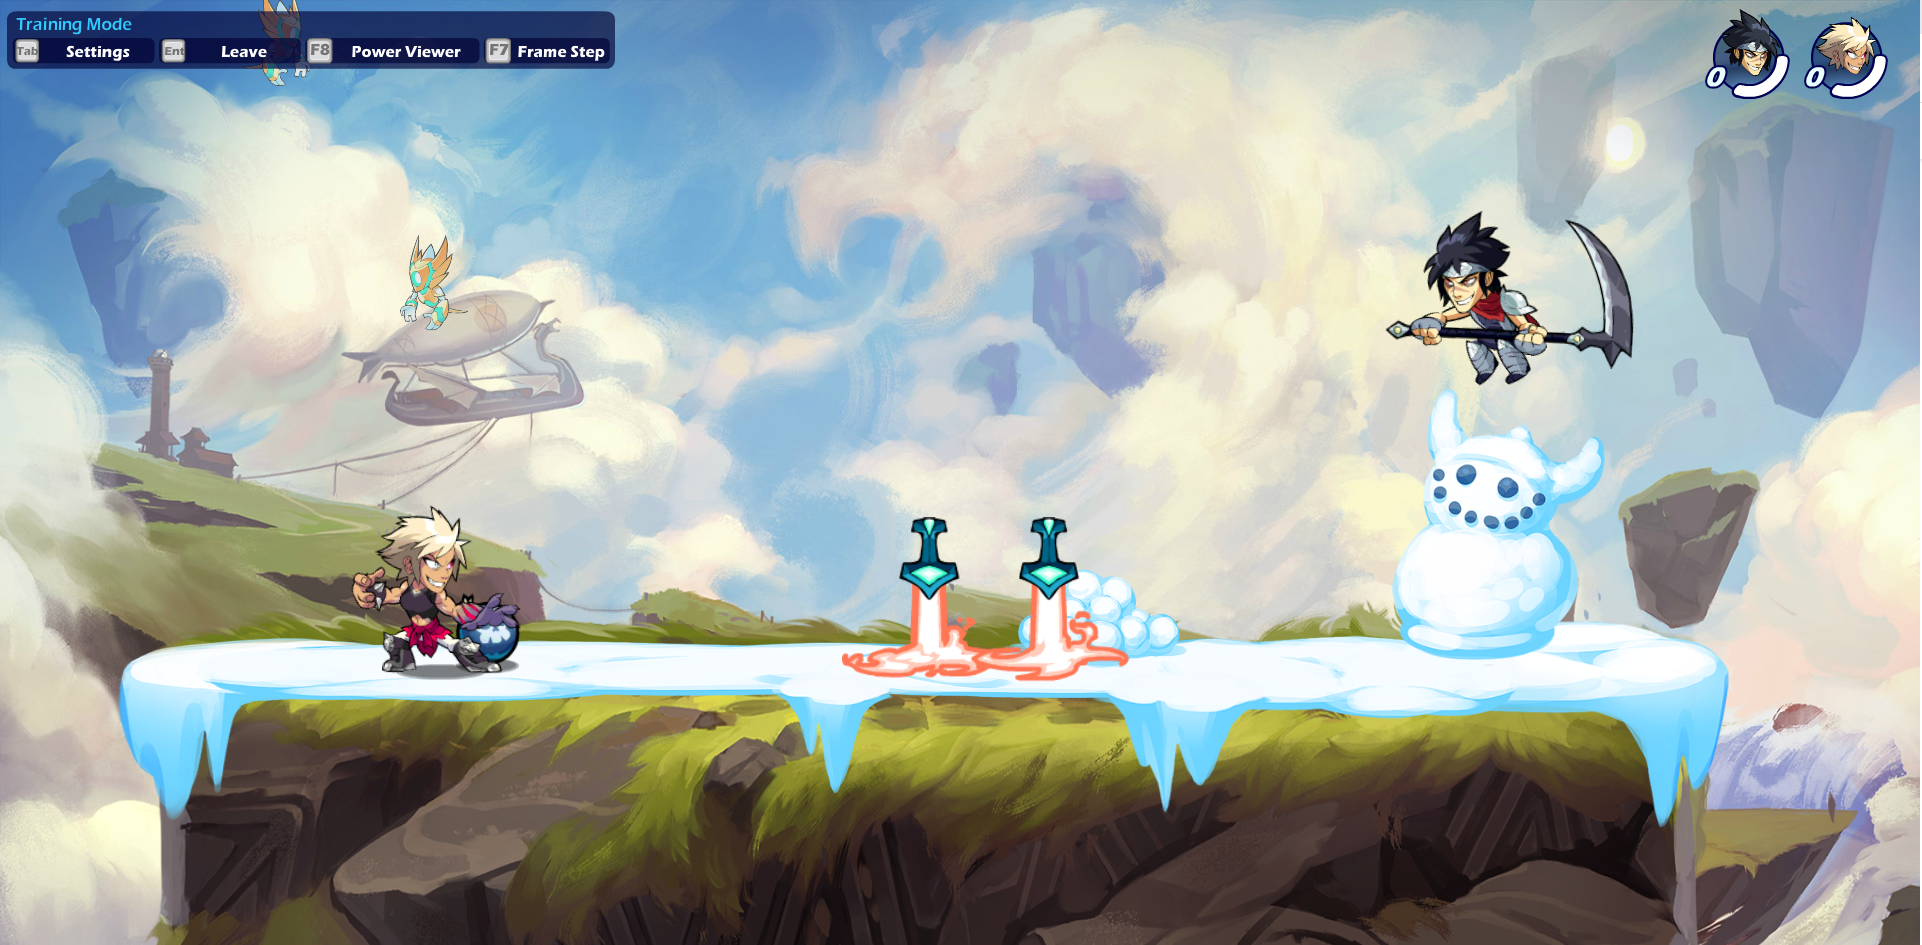
\includegraphics[scale=0.3]{pics/brawlhalla.PNG}
    \caption{Brawlhalla Spielumgebung}
    \label{fig:impl:knuth}
\end{figure}

Ein Nachteil hierbei ist, dass sich der Benutzer vor dem Spielen einen Account erstellen
und dann einen Download abschließen muss. Dazu kommt noch, dass die Spielumgebung nie beeinflusst werden kann.

\subsection{Stick Fight: The Game}
In diesem Spiel kämpfen die Spieler als Strichmännchen gegeneinander, die durch eine Ragdoll-Engine gesteuert werden, eine Engine, die das Bewegungsverhalten von menschlichen Körpern simuliert.
Auch wie bei schon bei vorher erwähnten Spielen, kann der Benutzer aber nicht einfach plattformunabhängig im Browser gegeneinander antreten.
Für die Spielekonsole Nintendo Switch zum Beispiel, gibt es das Spiel auch nicht. Hinzu kommt, dass auch die Umgebung nicht frei erstellt werden kann.

\section{Ist-Zustand}
Dadurch das es eine Diplomarbeit ist, fängt alles bei 0 an. Es gibt jedoch Frameworks,
welche die Erarbeitung erleichtern. Zum Beispiel im Falle des Spiels, welches
mittels Webtechnologien umgesetzt wird, kann p5.js verwendet werden, welches die
Umsetzung eines Spiels erleichtert. Ein weiteres Beispiel ist die Objekterkennung für
die Spielumgebung (Map). Diese wird von Open-CV übernommen.